\section{Exercise two}
Consider the ARMA(1, 1) process:
\[v(t)=\dfrac{1}{2}v(t-1)+\eta(t)-\eta(t-1) \qquad \eta(\cdot)\sim WN(1,9)\]
Compute the expected value and the variance.

\subsection{Solution}
The expected value is zero. 
The variance is:
\begin{align*}
    \gamma(0)=\text{Var}\left[v(t)\right] &= \mathbb{E}\left[(v(t) - 0)^2\right] \\
                                &= \mathbb{E}\left[(\dfrac{1}{2}v(t-1)+\eta(t)-\eta(t-1))^2\right]
\end{align*}
Expanding, we get:
\begin{multline*}
    \text{Var}\left[v(t)\right]= \dfrac{1}{4}\underbrace{\mathbb{E}\left[v(t-1)^2\right]}_{\text{Var}\left[v(t)\right]}  + \underbrace{\mathbb{E}\left[\eta(t)^2\right]}_{10}  -\underbrace{\mathbb{E}\left[\eta(t-1)^2\right]}_{10}  + \underbrace{\mathbb{E}\left[v(t-1)\eta(t)\right]}_{0} - \\ - \underbrace{\mathbb{E}\left[v(t-1)\eta(t-1)\right]}_{9}  - 2 \underbrace{\mathbb{E}\left[\eta(t)\eta(t-1)\right]}_{1}                           
\end{multline*}
Given that $\text{Var}[v(t)] = \text{Var}[v(t-1)] = \gamma(0)$ and $\text{Var}[\eta(t)] = \text{Var}[\eta(t-1)] = 9$, we have:
\[\text{Var}\left[v(t)\right]=\text{Var}\left[v(t)\right]+10-10-9-2\rightarrow\text{Var}\left[v(t)\right]=12\]
Additionally, we have:
\begin{itemize}
    \item $\gamma(1)=-3$. 
    \item $\gamma(2)=-\frac{3}{2}$. 
\end{itemize}
For $|\tau| \geq 2$, we have:
\[\gamma(\tau)=\left( \dfrac{1}{2} \right)^{\left\lvert \tau \right\rvert -1}\gamma(1)\]
The correlation function and the spectrum remain unchanged when we depolarize the process. 
Defining:
\[\tilde{v}(t)=v(t)-\mathbb{E}\left[v(t)\right]=v(t)\]
\[\tilde{\eta}(t)=\eta(t)-\mathbb{E}\left[\eta(t)\right]=\eta(t)-1\]
We obtain:
\[\tilde{v}(t)=\dfrac{1}{2}\tilde{v}(t-1)+\tilde{\eta}(t)-\tilde{\eta}(t-1) \qquad \tilde{\eta}(\cdot)\sim WN(0,9)\]

Using the transfer function: 
\[W(z)=\dfrac{1-z^{-1}}{1-\frac{1}{2}z^{-1}}\]
We can calculate the spectrum using the formula:
\[\Gamma_{\tilde{v}\tilde{v}}=\left\lvert W(e^{j\omega})\right\rvert^2\Gamma_\eta(\omega)=\frac{1-1\cos(\omega)}{1.25-\cos(\omega)}18 \]
This result in the following graph:
\begin{figure}[H]
    \centering
    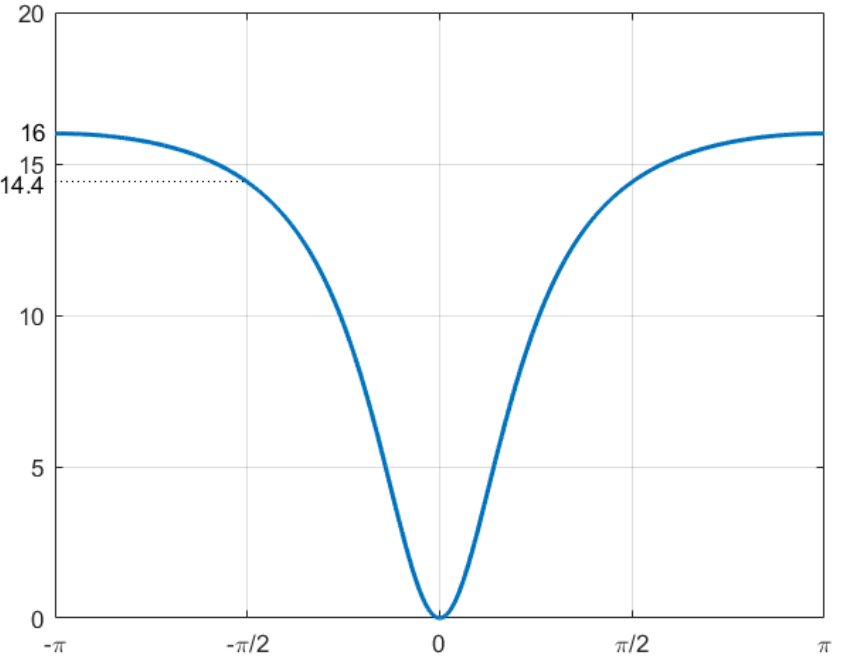
\includegraphics[width=0.5\linewidth]{images/22spec.png}
\end{figure}
The system blocks the component at zero frequency. 
Indeed, although the input has a non-zero mean, the output has null expected value.